\documentclass{article}
\usepackage[utf8]{inputenc}
\usepackage[T1]{fontenc}
\usepackage{amsmath}
\usepackage{amsfonts}
\usepackage{amssymb}
\usepackage{graphicx}
\usepackage{lipsum} 
\usepackage{hyperref}
\usepackage{algorithm}
\usepackage{algpseudocode}
\usepackage{pdfpages}

\title{Statistics Exercise 02}
\author{Enrico Cotti Cottini \\ Università di Padova \\ Matricola 2077993}
\date{\today}

\begin{document}

\maketitle

\section{Esercizio 15 }
In un ballottaggio tra due candidati, A e B, votano $N + M$ persone, con $N \in \mathbb{N}$, $M \in \{0, \ldots, N\}$: $N$ elettori sono completamente indecisi e votano a caso, senza preferenza tra A e B, mentre il gruppo di $M$ persone sostiene il candidato A. Vogliamo trovare la probabilità che vinca A.

Possiamo descrivere il comportamento elettorale delle $N$ persone indecise tramite una variabile aleatoria $S_N$ con distribuzione binomiale di parametri $N$ e $1/2$, definita su un opportuno spazio di probabilità $(\Omega, \mathcal{F}, P)$; $S_N$ rappresenta il numero di voti che il candidato A riceve dal gruppo delle persone indecise. La probabilità che vinca A è allora data da
\[
P\left( S_N + M > \frac{N + M}{2} \right) = P\left( S_N > \frac{N - M}{2} \right) = \sum_{k = \left\lfloor \frac{N - M}{2} \right\rfloor + 1}^{N} \text{pBin}\left(N, \frac{1}{2}\right)(k).
\]

Si scriva un programma che calcoli numericamente questa probabilità in funzione di $N$, $M$ come sopra, in grado di trattare il caso $N + M = 10^6$, $M \leq 5000$.

\subsection*{Per la consegna servono:}
\begin{itemize}
    \item lo svolgimento dell'Esercizio 14 e una giustificazione matematica della procedura utilizzata per il calcolo della probabilità di vittoria elettorale richiesta;
    \item lo pseudo-codice del programma e il codice commentato in un linguaggio standard come C++ o Python (il codice anche in un file separato);
    \item un grafico in formato PDF che riporti la probabilità di vittoria elettorale in funzione di $M$ quando $N + M = 10^6$ e $M$ varia da 0 a 5000 (in passi da dieci).
\end{itemize}

\section{Scelta e giustificazioni della procedura}
In un ballottaggio tra due candidati, A e B, abbiamo $N + M$ persone votanti in totale, dove $N$ elettori sono completamente indecisi, mentre il gruppo di $M$ persone sostiene il candidato A.

il comportamento elettorale delle $N$ persone indecise è descritto tramite una variabile aleatoria $S_N$ con distribuzione binomiale di parametri $N$ e $1/2$, questo vuol dire che le $N$ persone indecise corrispondono a $N$ tentativi ciascuno dei quali ha una possibilità di  $1/2$ di avverarsi, quindi $S_N$ equivale al numero di successi di un'estrazione di $N$ tentativi consecutivi, di cui come gia detto, ognuno ha possibiliyà $1/2$ di avverarsi.

Dunque la probabilità $P(A)$ ovvero la probabilità che $A$ vinca le elezioni  equivale alla probabilita che $ S_N + M$ (i votanti di A) sia
Maggiore alla metà del numero totale dei votanti $\frac{N + M}{2}$, ossia:
\[
P\left( S_N + M > \frac{N + M}{2} \right)
\]
che equivale a
\[
 P\left( S_N > \frac{N - M}{2} \right)
\]
Noi sappiamo che La funzione di massa di probabilità( funzione di massa perchè $S_N$ è una variabile aleatoria discreta dato che $N$ è un valore finito, Dimostrata alla fine del foglio della lezione del 25 marzo 2024 ) per $S_N$ di paramtri $(N,1/2)$ è data da:
\[
P(S_N = k) = \binom{N}{k} \frac{1}{2}^k (1-\frac{1}{2})^{N-k}
\]
dove 
\[
\binom{N}{k} = \frac{N!}{k!(N-k)!}
\]


La probabilità $P(S_N = x_i)$ può essere interpretata come la probabilità che $S_N$ assuma un valore specifico $x_i$ tra i possibili valori $x_1, x_2, \ldots, x_n$. 

Dire che $P\left( S_N > \frac{N - M}{2} \right)$ che equivale a sommare tutte le probabilità parziali $P(S_N = k_i)$ dove $k$ deve prendere i valori $k_i\in$ $\mathbb{N}$ maggiori di
$\frac{N - M}{2}$ fino al massimo che puo assumere $S_N $ ovvero $N$, quindi:
\[
\frac{N - M}{2} < k_1 = \frac{N - M}{2} + 1 < ... < k_n = N
\]
Quindi per ogni $K_i$ la funzione di massa diventa:
\[
\sum_{k = \left\lfloor \frac{N - M}{2} \right\rfloor + 1}^{N} \text{pBin}\left(N, \frac{1}{2}\right)(k) = \sum_{k = \left\lfloor \frac{N - M}{2} \right\rfloor + 1}^{N} P(S_N = k)
\]
\[
=
\sum_{k = \left\lfloor \frac{N - M}{2} \right\rfloor + 1}^{N} \binom{N}{k} \frac{1}{2}^k (1-\frac{1}{2})^{N-k} 
= \sum_{k = \left\lfloor \frac{N - M}{2} \right\rfloor + 1}^{N} \frac{N!}{k!(N-k)!} \frac{1}{2}^k (1-\frac{1}{2})^{N-k}
\]

Dunque in definitiva la probabilita che $A$ vinca $P(A)$ equivale a:
\[
P\left( S_N + M > \frac{N + M}{2} \right) = P\left( S_N > \frac{N - M}{2} \right) = \sum_{k = \left\lfloor \frac{N - M}{2} \right\rfloor + 1}^{N} \text{pBin}\left(N, \frac{1}{2}\right)(k).
\]
\[
=  \sum_{k = \left\lfloor \frac{N - M}{2} \right\rfloor + 1}^{N} \frac{N!}{k!(N-k)!} \frac{1}{2}^k (1-\frac{1}{2})^{N-k}
\]

\subsection{Considerazioni sulla complessita'}

Il problema principale di questa formula e' il calcolo del coeficiente binomiale 
\[
\binom{N}{k} = \frac{N!}{k!(N-k)!}
\]
questa operazione per N e k grandi diventa infattibile data la complessita' fattoriale O(n!) di questo calcolo sia in termini di tempo che di costo, quindi e' inpensabile l'utilizzo di questa formulazione per $N+M$ nell'ordine di $10^6$

\subsection{Soluzione possibile}

Cercando una soluzione a questo problema ho deciso di documentarmi sull' implementazione della funzione pmf (Probability Mass Function) e pdf(Probability density Function) della libreria Scipy di python, progetto open source distibuito con licenza BSD.

\href{https://github.com/scipy/scipy}{https://github.com/scipy/scipy}

La funzione PMF e' definita in stats/discrete distns.py come segue:

\begin{algorithm}
\caption{}
\begin{algorithmic}[1]
\Function{\_pmf}{$x, n, p$}
    \State \textbf{return} \_boost.\_binom\_pdf($x, n, p$)
\EndFunction
\end{algorithmic}
\end{algorithm}

Come possiamo vedere la libreria Boost viene utilizata ausiliariamente a Scipy e la vera implementazione di pdf(density) e' di Boost(libreria c++ opensource).

\newpage

in Boost la funzione pmf e':

\begin{algorithm}
\caption{}
\begin{algorithmic}[2]
\Function{pdf}{$\text{dist}, k$}
    \State \textbf{...} 
    \State \textbf{controlli} 
    \State \textbf{...} 

    \State \textbf{using} \textit{boost::math::ibeta\_derivative}
    \State \Return $\text{ibeta\_derivative}(k+1, n-k+1, \text{dist.success\_fraction()}) / (n+1)$
\EndFunction
\end{algorithmic}
\end{algorithm}


\begin{figure}[h]
  \centering
  \includegraphics[width=1\textwidth]{images/Schermata del 2024-04-02 17-05-24.png}
  \caption{commento sul codice.}
  \label{fig:your_image}
\end{figure}

Nelle righe commentate e' presente la formulazione matematica per esprimere la funzione pmf senza il coeficente binomiale e con la derivata della funzione beta incompleta, sarebbe:

\begin{align*}
& f(k; n,p) = C(n, k) \cdot p^k \cdot (1-p)^{n-k} \\
& \quad = \frac{n!}{k!(n-k)!} \cdot p^k \cdot (1-p)^{n-k} \\
& \quad = \frac{\Gamma(n+1)}{\Gamma(k+1)\Gamma(n-k+1)} \cdot p^k \cdot (1-p)^{n-k} \\
& \quad = p^k (1-p)^{n-k} / \left(\beta(k+1, n-k+1) \cdot (n+1)\right) \\
& \quad = \text{ibeta\_derivative}(k+1, n-k+1, p) / (n+1) \\
\end{align*}

Dove sono presenti:
\begin{enumerate}
    \item Il coefficiente binomiale $C(n,k)$.
    
    \item Il fattoriale $n!$,
    
    \item La funzione gamma $\Gamma(x)$, che generalizza il concetto di fattoriale ai numeri reali e complessi.

    
    \item $\beta(x,y)$ rappresenta la funzione beta, che è la funzione integrale della distribuzione beta.
    
    \item La funzione $\text{ibeta\_derivative}(a,b,x)$ rappresenta la derivata parziale della funzione beta incompleta.
\end{enumerate}

Quindi questa formulazione utilizza la derivata parziale della funzione beta incompleta e la funzione beta incompleta.

\subsection{Implementazione}

L'implementazione delle funzioni beta incomplete nelle librerie Boost C++ si basa sull'Algoritmo 708, intitolato "Significant digit computation of the incomplete beta function ratios" di DiDonato e Morris. Queste funzioni calcolano la funzione beta incompleta.

spiegazione semplificata di questa implementazione:

\begin{enumerate}
  \item \textbf{Implementazione Comune}: Tutte e quattro le funzioni condividono un'implementazione comune, che riceve sia $x$ che $y$. A seconda della situazione, può essere restituito $p$ o $q$, dove $p$ e $q$ sono correlati.
  
  \item \textbf{Frazione Continua}: Sono utilizzate diverse rappresentazioni di frazioni continue in base ai valori di $a$ e $b$:
    \begin{itemize}
      \item Una frazione continua che si trova sui libri di testo è disponibile ma non utilizzata nell'implementazione a causa di problemi di velocità e accuratezza.
      \item Quando sia $a$ che $b$ sono maggiori di 1, viene utilizzata una frazione continua di DiDonato e Morris.
      \item Per valori piccoli di $b$ e $x$, viene utilizzata una rappresentazione in serie.
      \item Quando $b$ è molto più piccolo di $a$, viene utilizzata una rappresentazione in serie con una funzione gamma incompleta.
    \end{itemize}

\end{enumerate}

L'implementazione seleziona il metodo appropriato in base ai valori di $a$, $b$ e $x$.

Per documentazione piu approfondita :

\begin{enumerate}
  \item Boost C++ Libraries:
    \begin{itemize}
      \item \href{https://www.boost.org/doc/libs/1_84_0/libs/math/doc/html/math_toolkit/sf_beta/beta_derivative.html}{Beta Derivative}
      \item \href{https://www.boost.org/doc/libs/1_84_0/libs/math/doc/html/math_toolkit/sf_beta/ibeta_function.html}{Incomplete Beta Function}
    \end{itemize}
  
  \item Wikipedia:
    \begin{itemize}
      \item \href{https://en.wikipedia.org/wiki/Beta_function}{Beta Function}
      \item \href{https://en.wikipedia.org/wiki/Incomplete_beta_function}{Incomplete Beta Function}
    \end{itemize}
  
  \item Wolfram MathWorld:
    \begin{itemize}
      \item \href{https://mathworld.wolfram.com/IncompleteBetaFunction.html}{Incomplete Beta Function}
    \end{itemize}
  
  \item SciPy Documentation:
    \begin{itemize}
      \item \href{https://docs.scipy.org/doc/scipy/reference/generated/scipy.special.betainc.html}{scipy.special.betainc}
    \end{itemize}
  
  \item DLMF (Digital Library of Mathematical Functions):
    \begin{itemize}
      \item \href{https://dlmf.nist.gov/8.17}{Incomplete Beta Function}
    \end{itemize}
\end{enumerate}

\section{pseudo-codice}

Nel file PMF.py ho implementato 2 funzioni pmf che associano a ciascun valore di una variabile aleatoria discreta la probabilità che la variabile aleatoria assuma quel valore.
la prima pmf calcola la probabilita' utilizzando la formula sopracitata che utilizza la derivata della funzione beta incompleta betainc() la quale e' a sua volta implementata dalla libreria scipy. La seconda scipy\_pmf utilizza direttamente binom.pmf la funzione pmf implementata dalla libreria scipy.
\newline
Ho fatto queste due distinzioni perche' la funzione pmf e' molto piu rapida della seconda probabilmente per qualche differenza di implementazione interna della libreria scipy.
\newline 
L'esecuzione del programma con la prima funzione impiega circa 12 secondi sulla mia macchina mentre la seconda impiega circa 300 secondi.
\begin{algorithm}
\caption{Calcolo della funzione di massa di probabilità (PMF) tramite derivata della funzione beta incompleta}
\begin{algorithmic}[3]
\Function{ibeta\_derivative}{$a, b, x, h=1e-5$}
    \State $fx \gets \text{betainc}(a, b, x)$
    \State $fx\_plus\_h \gets \text{betainc}(a, b, x + h)$
    \State $\text{derivative} \gets \frac{{fx\_plus\_h - fx}}{h}$
    \State \Return $\text{derivative}$
\EndFunction

\Function{pmf}{$n, k, p$}
    \State $\text{ibeta\_deriv} \gets \text{ibeta\_derivative}(k + 1, n - k + 1, p)$
    \State $\text{pmf} \gets \frac{{\text{ibeta\_deriv}}}{{n + 1}}$
    \State \Return $\text{pmf}$
\EndFunction

\Function{scipy\_pmf}{$n, k, p$}
    \State $\text{pmf\_value} \gets \text{binom.pmf}(k, n, p)$
    \State \Return $\text{pmf\_value}$
\EndFunction
\end{algorithmic}
\end{algorithm}

Nel file main.py e' presente il codice per la sommatoria delle probabilita' che compongono la probabilita della vittoria di A, in piu' questa probabilita' viene calcolata n volte per diversi valori di M ( compresi tra 0 e 5000 ) dove n = step.
E poi il codice per plottare il risultato.

\begin{algorithm}
\caption{Calcolo di A\_win}
\begin{algorithmic}[1]
\Function{dada}{asdad}
\State $N+M = 1000000$
\State $M\_values = \text{np.linspace}(0, M_{\text{max}}, \text{step}, \text{dtype}=\text{int})$
\State $N\_values = N+M - M\_values$
\State $p = 0.5$

    \For{$(M,N)$ in \text{zip}$(M\_values, N\_values - M\_values)$}
        \State $k\_values = \text{np.arange}\left(\left\lfloor\frac{{N - M}}{2}\right\rfloor + 1, N\right)$

        \State $p\_A = \sum_{k = \left\lfloor \frac{N - M}{2} \right\rfloor + 1}^{N} pmf(N, k, p) $

    \EndFor

\EndFunction
\end{algorithmic}
\end{algorithm}


\section{Grafico N+M in funzione di M crescente}
grafico in formato PDF che riporti la probabilità di vittoria elettorale
in funzione di M quando N + M = 1000000 e M varia da 0 a 5000
Possiamo osservare che con l'aumentare dei Votanti sicuri di M allora la probabilita' della vittoria di A aumenta fino a stabilizzarsi su un valore vicino al 100\%
pagina successiva

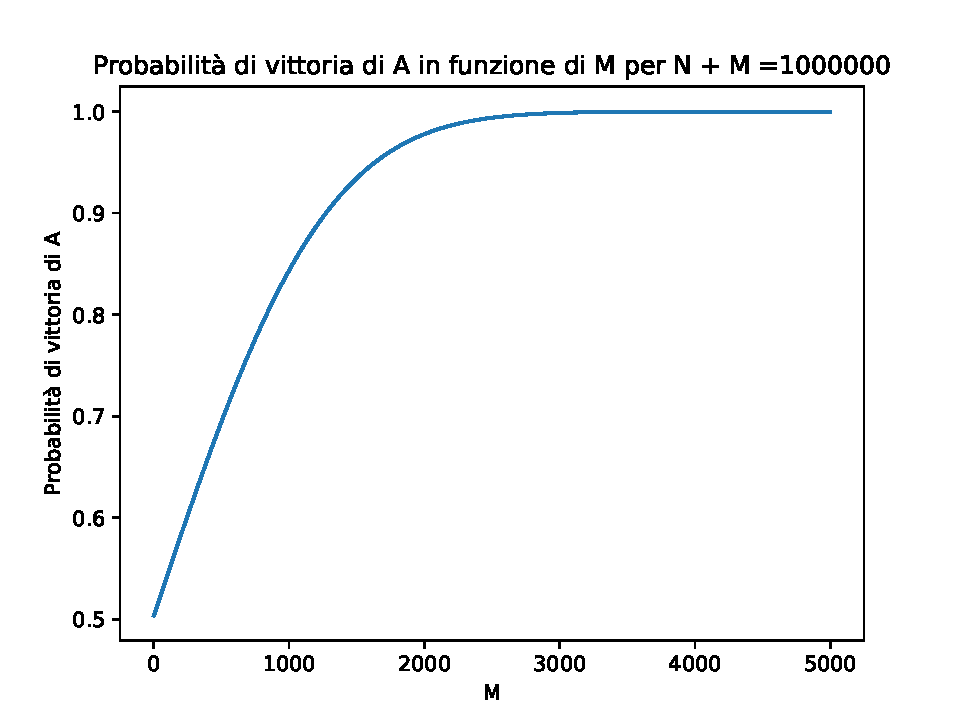
\includepdf[pages=-,  scale=1]{P_A.pdf}





\end{document}

